% !TEX root = ..\thesis.tex


 







\chapter{ Mô hình}
% vẽ sơ đồ hệ thống

\chapter{Đoạn của Quyết}
\section{Giới thiệu}
Một quy trình xử lý rác thải sẽ bao gồm rất nhiều công đoạn: thu gôm, phân loại và xử lý rác thải.
Cũng đã có các biện pháp để giảm bớt quá trình phân loại rác bằng cách đặt thùng rác dán sẵn nhãn phân loại tương ứng để người sử dụng phân biệt.
Tuy nhiên, thực tế cho thấy, biện pháp này chưa thực sự giải quyết triệt để vấn đề trên. 
Nên việc thay thế cách phân loiaj truyền thống bằng các thùng rác tự động phân loại là biện pháp khả thi hơn.
Bằng việc lấy các tập dữ liệu lớn có sẵn sẽ làm tăng tính chính xác cho sản phẩm. 

\section{Giới thiệu về model CNN}
Mạng CNN là một tập hợp các lớp Convolution chồng lên nhau và sử dụng các hàm nonlinear activation như ReLU và tanh để kích hoạt các trọng số trong các node. 
CNN được dùng trong trong nhiều bài toán như nhân dạng ảnh, phân tích video, ảnh MRI, hoặc cho bài các bài của lĩnh vự xử lý ngôn ngữ tự nhiên. Trong đề tài này, chúng tôi đã sử dụng mạng CNN để giải quyết bài toán phân loại rác.

Bài toán có đầu vào là một hình ảnh của rác được đưa vào thùng và đầu ra là nhãn của loại rác đó.
%(từ camera của thiết bị hay cái gì đó cụ thể hơn nha)% 
CNN bao gồm tập hợp các lớp cơ bản bao gồm: convolution layer + nonlinear layer, pooling layer, fully connected layer. 
Các lớp này liên kết với nhau theo một thứ tự nhất định. Thông thường, một ảnh sẽ được lan truyền qua tầng convolution layer + nonlinear layer đầu tiên, sau đó các giá trị tính toán được sẽ lan truyền qua pooling layer, bộ ba convolution layer + nonlinear layer + pooling layer có thể được lặp lại nhiều lần trong network. Và sau đó được lan truyền qua tầng fully connected layer và softmax để tính xác suất ảnh đó chứa vật thế gì.
% Cái lý thuyết khúc này thì thêm sau nha, tùy vào thầy muốn cụ thể đến mức nào, có bắt giải thích từng lớp trong mạng là gì hay không

\subsection{Tối ưu model để có thể chạy trên được chip nhúng ESP32}
% phần code 
\begin{figure}[ht]
    \centering
    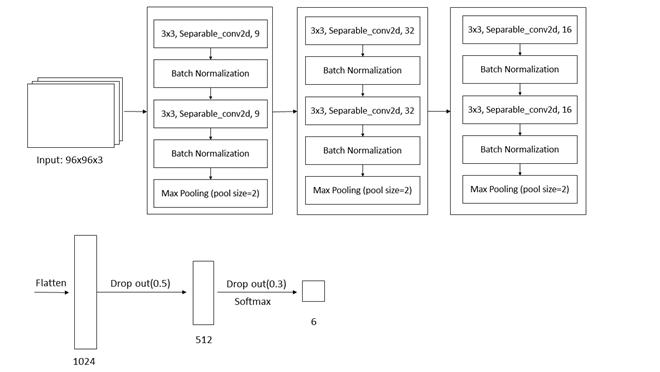
\includegraphics[width=\linewidth]{images/ktmang.png}
    \caption{ Minh họa kiến trúc mạng đã xây dựng}
    \label{fig:kientrucmang}
\end{figure}
% Do chip nhúng gì đó chỉ có bao nhiêu ram đó nên chúng tôi không thể xây dựng mô hình với trong số quá lớn và có chi phí tính toán cao được, nên chúng tôi sử dụng ...(thêm đoạn sau vô nè)
% Thêm dụ giảm kích thước của hình ảnh từ bao nhiêu đó xuống 96 * 96 nữa nà
Sử dụng separable convolution thay cho lớp convolution thông thường để giảm bớt chi phí tính toán cho mạng. Ngoài ra ở lớp này, chúng tôi dùng regularization l2 để tránh overfitting và hàm kích hoạt relu – đây là hàm thường được sử dụng trong quá trình train model với dữ liệu dưới dạng ảnh. Chúng tôi cũng thêm các lớp batch normalization và drop out để tránh cho mô hình bị overfitting và loại bỏ sự kết nối chặt chẽ giữa các lớp fully connected. Tổng số tham số của mô hình là 532,161. Sau khi xây dụng mô hình, nhóm đã sử dụng optimization stochastic gradient descent với learning rate = 1e-4 và momentum = 0.8 để train mô hình.

\section{Evaluation}
\subsection{Data Description} % Giới thiệu về dataset ddùng để train và test 
% Dữ liệu được lấy từ cái gì đó quên oy, nhưng cái này nên thêm vô nha
% Kích thước của hình là ... không nhớ a
Gồm 2527 hình thuộc 6 lớp với sự phận bố ở mỗi lớp:
 
Cardboard: 403

Glass: 501

Metal: 410

Paper: 594

Plastic: 482

Trash: 137
 
Dữ liệu được chia làm 2 phần theo tỉ lệ 80\% train và 20\% test.

Train: 2024

Test: 503
% Nên lựa vài hình về data để thêm vô (nếu cần) hình nên có đủ 6 lớp cần phân loại
\subsection{Index of Performance} % Các chỉ số để dánh gia model  %accuracy, F-score - Recall.
Chúng tôi sử dụng hai chỉ số là accuracy và F1-score để đánh giá model. Accuracy là tính tỉ lệ giữa số ảnh được dự đoán đúng và tổng số ảnh trong tập dữ liệu kiểm thử.
% Còn khúc giới thiệu F1 nữa cơ mà đang lười ghi công thức toán trong đây nha
% Khúc này thêm lý thuyết của hai cái chỉ số đó
\subsection{Results} % Kết quả  hiện thực được 
Kết quả train mô hình với 80 epoch
\begin{figure}[ht]
    \centering
    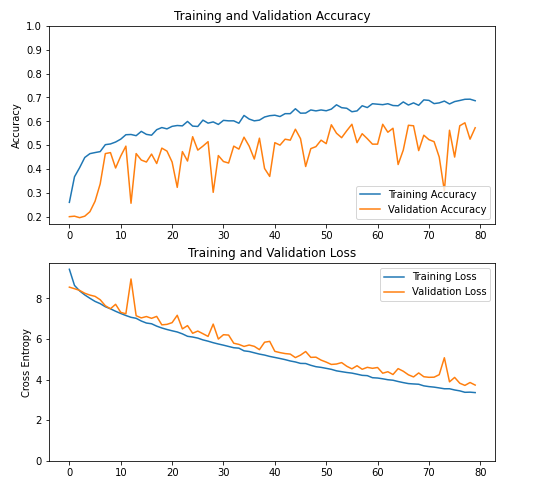
\includegraphics[width=\linewidth]{images/graph.png}
    \caption{ Biểu đồ thể hiện loss và accuracy của mô hình trong quá trình train}
    \label{fig:graph}
\end{figure}
% Hai cái này nên chuyển thành dạng bảng, cơ mà đang lười chuyển
Accuracy cao nhất trên tập train là 0.6938 và trên tập test là 0.5938
Loss nhỏ nhất trên tập train là 3.3844 và trên tập test là 3.7116

Kết quả thử nghiệm mô hình trên tập test sau khi đã lưu mô hình tốt nhất từ quá trình train 
\begin{figure}[ht]
    \centering
    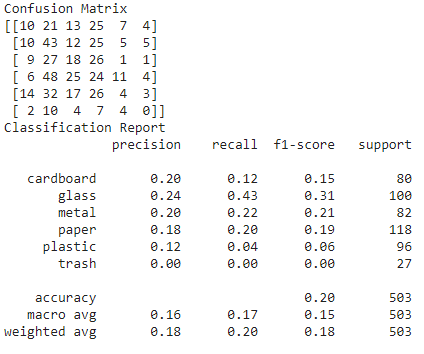
\includegraphics[width=\linewidth]{images/matrix.png}
    \caption{ Confusion matrix của model khi thử lại trên tập test}
    \label{fig:matrix}
\end{figure}
Từ hình \ref{fig:matrix} ta có thể thấy accuracy và f1-score của mô hình còn khá thấp, tuy nhiên do mô hình được xây dựng chỉ có 532,161 tham số nên không đủ để phân loại chính xác các lớp được. Chúng tôi đã thử train thêm epoch nhưng mô hình dễ bị overfitting và kết quả khi in confusion matrix vẫn không thay đổi nhiều. Ngoài ra nếu tăng thêm trọng số thì không thể sử dụng model trên thiết bị được.
